
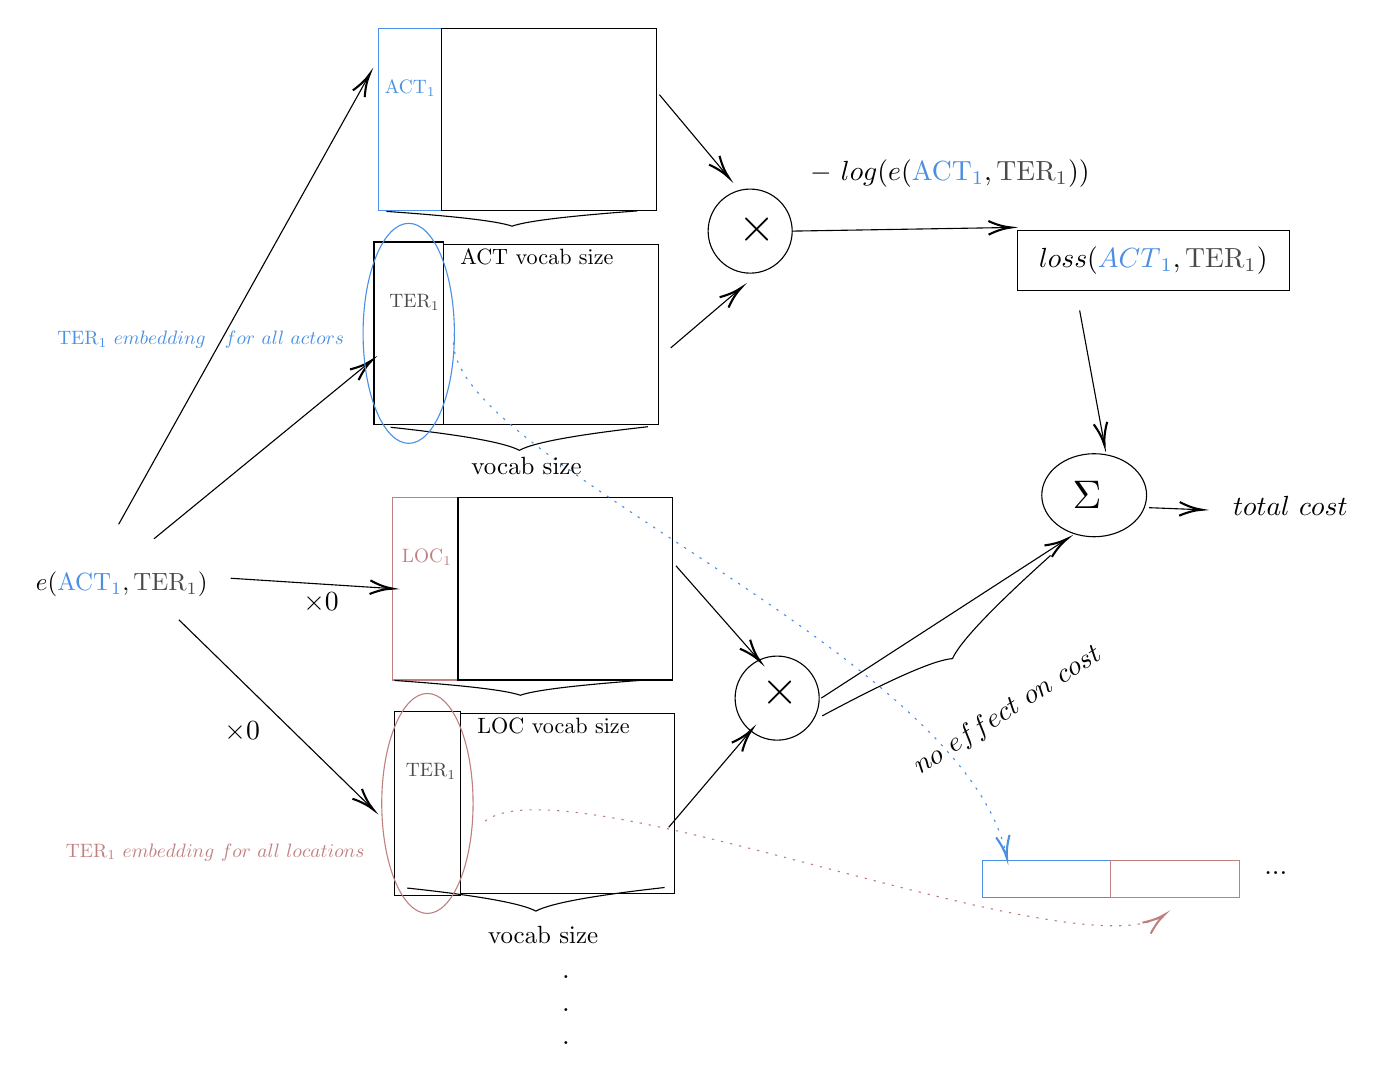
\begin{tikzpicture}[x=0.75pt,y=0.75pt,yscale=-1,xscale=1]
%uncomment if require: \path (0,547); %set diagram left start at 0, and has height of 547

%Straight Lines [id:da13430096728319052] 
\draw    (71.5,277) -- (174.95,192.27) ;
\draw [shift={(176.5,191)}, rotate = 500.68] [color={rgb, 255:red, 0; green, 0; blue, 0 }  ][line width=0.75]    (10.93,-3.29) .. controls (6.95,-1.4) and (3.31,-0.3) .. (0,0) .. controls (3.31,0.3) and (6.95,1.4) .. (10.93,3.29)   ;

%Straight Lines [id:da3395203365138022] 
\draw    (54.5,270) -- (174.53,54.75) ;
\draw [shift={(175.5,53)}, rotate = 479.14] [color={rgb, 255:red, 0; green, 0; blue, 0 }  ][line width=0.75]    (10.93,-3.29) .. controls (6.95,-1.4) and (3.31,-0.3) .. (0,0) .. controls (3.31,0.3) and (6.95,1.4) .. (10.93,3.29)   ;

%Shape: Rectangle [id:dp40988752111198234] 
\draw  [color={rgb, 255:red, 74; green, 144; blue, 226 }  ,draw opacity=1 ] (179.5,31) -- (210,31) -- (210,119) -- (179.5,119) -- cycle ;
%Shape: Rectangle [id:dp8120457242640955] 
\draw   (177.5,134) -- (211,134) -- (211,222) -- (177.5,222) -- cycle ;
%Shape: Rectangle [id:dp5994549314957651] 
\draw  [color={rgb, 255:red, 0; green, 0; blue, 0 }  ,draw opacity=1 ] (210,31) -- (313.5,31) -- (313.5,119) -- (210,119) -- cycle ;
%Shape: Rectangle [id:dp8953379233256253] 
\draw  [color={rgb, 255:red, 0; green, 0; blue, 0 }  ,draw opacity=1 ] (211,135) -- (314.5,135) -- (314.5,222) -- (211,222) -- cycle ;
\draw   (309.5,223) .. controls (275.06,226.82) and (254.4,230.61) .. (247.52,234.37) .. controls (240.63,230.64) and (219.95,226.93) .. (185.5,223.26) ;
\draw   (304.5,119) .. controls (270.9,121.49) and (250.73,123.94) .. (244.02,126.37) .. controls (237.29,123.97) and (217.12,121.6) .. (183.5,119.25) ;
%Shape: Ellipse [id:dp16021666171497673] 
\draw   (338.5,128.75) .. controls (338.5,117.57) and (347.57,108.5) .. (358.75,108.5) .. controls (369.93,108.5) and (379,117.57) .. (379,128.75) .. controls (379,139.93) and (369.93,149) .. (358.75,149) .. controls (347.57,149) and (338.5,139.93) .. (338.5,128.75) -- cycle ;
%Straight Lines [id:da010832594540308715] 
\draw    (320.5,185) -- (352.98,157.3) ;
\draw [shift={(354.5,156)}, rotate = 499.54] [color={rgb, 255:red, 0; green, 0; blue, 0 }  ][line width=0.75]    (10.93,-3.29) .. controls (6.95,-1.4) and (3.31,-0.3) .. (0,0) .. controls (3.31,0.3) and (6.95,1.4) .. (10.93,3.29)   ;

%Straight Lines [id:da7904695547993323] 
\draw    (315,63) -- (347.22,101.47) ;
\draw [shift={(348.5,103)}, rotate = 230.05] [color={rgb, 255:red, 0; green, 0; blue, 0 }  ][line width=0.75]    (10.93,-3.29) .. controls (6.95,-1.4) and (3.31,-0.3) .. (0,0) .. controls (3.31,0.3) and (6.95,1.4) .. (10.93,3.29)   ;

%Straight Lines [id:da40310566362864897] 
\draw    (517.5,167) -- (529.14,230.03) ;
\draw [shift={(529.5,232)}, rotate = 259.54] [color={rgb, 255:red, 0; green, 0; blue, 0 }  ][line width=0.75]    (10.93,-3.29) .. controls (6.95,-1.4) and (3.31,-0.3) .. (0,0) .. controls (3.31,0.3) and (6.95,1.4) .. (10.93,3.29)   ;

%Shape: Rectangle [id:dp7172146507008619] 
\draw  [color={rgb, 255:red, 191; green, 128; blue, 128 }  ,draw opacity=1 ] (186.5,257) -- (218,257) -- (218,345) -- (186.5,345) -- cycle ;
%Shape: Rectangle [id:dp060267406747659624] 
\draw   (187.5,360) -- (219,360) -- (219,449) -- (187.5,449) -- cycle ;
%Shape: Rectangle [id:dp6303673802072765] 
\draw  [color={rgb, 255:red, 0; green, 0; blue, 0 }  ,draw opacity=1 ] (218,257) -- (321.5,257) -- (321.5,345) -- (218,345) -- cycle ;
%Shape: Rectangle [id:dp304301296261714] 
\draw  [color={rgb, 255:red, 0; green, 0; blue, 0 }  ,draw opacity=1 ] (219,361) -- (322.5,361) -- (322.5,448) -- (219,448) -- cycle ;
\draw   (317.5,445) .. controls (283.06,448.82) and (262.4,452.61) .. (255.52,456.37) .. controls (248.63,452.64) and (227.95,448.93) .. (193.5,445.26) ;
%Shape: Ellipse [id:dp22428072345396544] 
\draw   (351.5,353.75) .. controls (351.5,342.57) and (360.57,333.5) .. (371.75,333.5) .. controls (382.93,333.5) and (392,342.57) .. (392,353.75) .. controls (392,364.93) and (382.93,374) .. (371.75,374) .. controls (360.57,374) and (351.5,364.93) .. (351.5,353.75) -- cycle ;
%Straight Lines [id:da29040700011246456] 
\draw    (319.5,416) -- (358.2,370.52) ;
\draw [shift={(359.5,369)}, rotate = 490.4] [color={rgb, 255:red, 0; green, 0; blue, 0 }  ][line width=0.75]    (10.93,-3.29) .. controls (6.95,-1.4) and (3.31,-0.3) .. (0,0) .. controls (3.31,0.3) and (6.95,1.4) .. (10.93,3.29)   ;

%Straight Lines [id:da7545042977801857] 
\draw    (323,290) -- (362.18,334.5) ;
\draw [shift={(363.5,336)}, rotate = 228.64] [color={rgb, 255:red, 0; green, 0; blue, 0 }  ][line width=0.75]    (10.93,-3.29) .. controls (6.95,-1.4) and (3.31,-0.3) .. (0,0) .. controls (3.31,0.3) and (6.95,1.4) .. (10.93,3.29)   ;

%Straight Lines [id:da13418076605656504] 
\draw    (393,353.75) -- (509.82,278.09) ;
\draw [shift={(511.5,277)}, rotate = 507.07] [color={rgb, 255:red, 0; green, 0; blue, 0 }  ][line width=0.75]    (10.93,-3.29) .. controls (6.95,-1.4) and (3.31,-0.3) .. (0,0) .. controls (3.31,0.3) and (6.95,1.4) .. (10.93,3.29)   ;

\draw   (308.5,345) .. controls (274.9,347.49) and (254.73,349.94) .. (248.02,352.37) .. controls (241.29,349.97) and (221.12,347.6) .. (187.5,345.25) ;
%Shape: Ellipse [id:dp1891084828946663] 
\draw  [color={rgb, 255:red, 74; green, 144; blue, 226 }  ,draw opacity=1 ] (172.25,178) .. controls (172.25,148.73) and (182.1,125) .. (194.25,125) .. controls (206.4,125) and (216.25,148.73) .. (216.25,178) .. controls (216.25,207.27) and (206.4,231) .. (194.25,231) .. controls (182.1,231) and (172.25,207.27) .. (172.25,178) -- cycle ;
%Shape: Ellipse [id:dp5133297466247488] 
\draw  [color={rgb, 255:red, 191; green, 128; blue, 128 }  ,draw opacity=1 ] (181.25,404.5) .. controls (181.25,375.23) and (191.1,351.5) .. (203.25,351.5) .. controls (215.4,351.5) and (225.25,375.23) .. (225.25,404.5) .. controls (225.25,433.77) and (215.4,457.5) .. (203.25,457.5) .. controls (191.1,457.5) and (181.25,433.77) .. (181.25,404.5) -- cycle ;
%Shape: Rectangle [id:dp8154703521346762] 
\draw  [color={rgb, 255:red, 74; green, 144; blue, 226 }  ,draw opacity=1 ] (470.5,432) -- (532.5,432) -- (532.5,450) -- (470.5,450) -- cycle ;
%Shape: Rectangle [id:dp3576905019222951] 
\draw  [color={rgb, 255:red, 191; green, 128; blue, 128 }  ,draw opacity=1 ] (532.5,432) -- (594.5,432) -- (594.5,450) -- (532.5,450) -- cycle ;
%Straight Lines [id:da3207889104512305] 
\draw    (108.5,296) -- (184.5,300.87) ;
\draw [shift={(186.5,301)}, rotate = 183.67] [color={rgb, 255:red, 0; green, 0; blue, 0 }  ][line width=0.75]    (10.93,-3.29) .. controls (6.95,-1.4) and (3.31,-0.3) .. (0,0) .. controls (3.31,0.3) and (6.95,1.4) .. (10.93,3.29)   ;

%Straight Lines [id:da444746435738554] 
\draw    (83.5,316) -- (175.82,406.1) ;
\draw [shift={(177.25,407.5)}, rotate = 224.3] [color={rgb, 255:red, 0; green, 0; blue, 0 }  ][line width=0.75]    (10.93,-3.29) .. controls (6.95,-1.4) and (3.31,-0.3) .. (0,0) .. controls (3.31,0.3) and (6.95,1.4) .. (10.93,3.29)   ;

\draw   (503.5,285) .. controls (475.52,310.16) and (459.77,326.73) .. (456.25,334.71) .. controls (447.55,335.32) and (426.62,344.52) .. (393.47,362.3) ;
%Shape: Ellipse [id:dp6408782289262511] 
\draw   (499.25,256) .. controls (499.25,244.95) and (510.55,236) .. (524.5,236) .. controls (538.45,236) and (549.75,244.95) .. (549.75,256) .. controls (549.75,267.05) and (538.45,276) .. (524.5,276) .. controls (510.55,276) and (499.25,267.05) .. (499.25,256) -- cycle ;
%Straight Lines [id:da19133214528940812] 
\draw    (379,128.75) -- (482.5,127.03) ;
\draw [shift={(484.5,127)}, rotate = 539.05] [color={rgb, 255:red, 0; green, 0; blue, 0 }  ][line width=0.75]    (10.93,-3.29) .. controls (6.95,-1.4) and (3.31,-0.3) .. (0,0) .. controls (3.31,0.3) and (6.95,1.4) .. (10.93,3.29)   ;

%Straight Lines [id:da406862365844594] 
\draw    (551,262) -- (574.5,262.92) ;
\draw [shift={(576.5,263)}, rotate = 182.25] [color={rgb, 255:red, 0; green, 0; blue, 0 }  ][line width=0.75]    (10.93,-3.29) .. controls (6.95,-1.4) and (3.31,-0.3) .. (0,0) .. controls (3.31,0.3) and (6.95,1.4) .. (10.93,3.29)   ;

%Curve Lines [id:da14396608756415818] 
\draw [color={rgb, 255:red, 191; green, 128; blue, 128 }  ,draw opacity=1 ] [dash pattern={on 0.84pt off 2.51pt}]  (231,413) .. controls (270.6,383.3) and (513.57,485.91) .. (557.24,458.86) ;
\draw [shift={(558.5,458)}, rotate = 503.13] [color={rgb, 255:red, 191; green, 128; blue, 128 }  ,draw opacity=1 ][line width=0.75]    (10.93,-3.29) .. controls (6.95,-1.4) and (3.31,-0.3) .. (0,0) .. controls (3.31,0.3) and (6.95,1.4) .. (10.93,3.29)   ;

%Curve Lines [id:da8005082280810756] 
\draw [color={rgb, 255:red, 74; green, 144; blue, 226 }  ,draw opacity=1 ] [dash pattern={on 0.84pt off 2.51pt}]  (216.25,178) .. controls (203.56,234.72) and (460.91,329.05) .. (482.2,429.49) ;
\draw [shift={(482.5,431)}, rotate = 259.35] [color={rgb, 255:red, 74; green, 144; blue, 226 }  ,draw opacity=1 ][line width=0.75]    (10.93,-3.29) .. controls (6.95,-1.4) and (3.31,-0.3) .. (0,0) .. controls (3.31,0.3) and (6.95,1.4) .. (10.93,3.29)   ;


% Text Node
\draw (195,60) node [scale=0.7,color={rgb, 255:red, 74; green, 144; blue, 226 }  ,opacity=1 ]  {$\mathrm{ACT}_{1}$};
% Text Node
\draw (362,128) node [scale=1.7280000000000002]  {$\times $};
% Text Node
\draw (197,163) node [scale=0.7,color={rgb, 255:red, 74; green, 74; blue, 74 }  ,opacity=1 ]  {$\mathrm{TER}_{1}$};
% Text Node
\draw (256,141) node [scale=0.8] [align=left] {ACT vocab size};
% Text Node
\draw (251,242) node [scale=0.9] [align=left] {vocab size};
% Text Node
\draw (203,286) node [scale=0.7,color={rgb, 255:red, 191; green, 128; blue, 128 }  ,opacity=1 ]  {$\mathrm{LOC}_{1}$};
% Text Node
\draw (205,389) node [scale=0.7,color={rgb, 255:red, 74; green, 74; blue, 74 }  ,opacity=1 ]  {$\mathrm{TER}_{1}$};
% Text Node
\draw (264,367) node [scale=0.8] [align=left] {LOC vocab size};
% Text Node
\draw (259,468) node [scale=0.9] [align=left] {vocab size};
% Text Node
\draw (270,504) node  [align=left] {.\\.\\.};
% Text Node
\draw (94,181) node [scale=0.7,color={rgb, 255:red, 74; green, 144; blue, 226 }  ,opacity=1 ]  {$\mathrm{TER}_{1} \ embedding\ \ \ for\ all\ actors$};
% Text Node
\draw (101,428) node [scale=0.7,color={rgb, 255:red, 191; green, 128; blue, 128 }  ,opacity=1 ]  {$\mathrm{TER}_{1} \ embedding\ for\ all\ locations$};
% Text Node
\draw (612,438) node  [align=left] {...};
% Text Node
\draw (114,370) node   {$\times 0$};
% Text Node
\draw (152,308) node   {$\times 0$};
% Text Node
\draw (483,360) node [rotate=-327.48]  {$ \begin{array}{l}
no\ effect\ on\ cost\\
\end{array}$};
% Text Node
\draw (521,256) node [scale=1.44]  {$\Sigma $};
% Text Node
\draw (373,351) node [scale=1.7280000000000002]  {$\times $};
% Text Node
\draw (56,299) node [scale=0.9] [align=left] {$e (\textcolor[rgb]{0.29,0.56,0.89}{\mathrm{ACT}}\textcolor[rgb]{0.29,0.56,0.89}{_{1}} ,\textcolor[rgb]{0.29,0.29,0.29}{\mathrm{TER}_{1}})$};
% Text Node
\draw    (487.5,128.5) -- (618.5,128.5) -- (618.5,157.5) -- (487.5,157.5) -- cycle  ;
\draw (553,143) node  [align=left] {$loss(\textcolor[rgb]{0.29,0.56,0.89}{ACT}\textcolor[rgb]{0.29,0.56,0.89}{_{1}} ,\textcolor[rgb]{0.29,0.29,0.29}{\mathrm{TER}_{1}})$};
% Text Node
\draw (455,101) node  [align=left] {$-\ log( e (\textcolor[rgb]{0.29,0.56,0.89}{\mathrm{ACT}}\textcolor[rgb]{0.29,0.56,0.89}{_{1}} ,\textcolor[rgb]{0.29,0.29,0.29}{\mathrm{TER}_{1}}))$};
% Text Node
\draw (619,261) node  [align=left] {$total\ cost$};


\end{tikzpicture}